\chapter{Language Recognition Systems}

\section{Language Detection vs. Identification}
\label{sect:detvsid}

Identification and detection of languages are two very related tasks in language recognition. In both tasks languages are constricted to be in a set of classes. Each class can be a single language, dialect, or a set of languages, and the goal of our system is to separate these classes. In this thesis we will only look at formulations where each class is a single language and possibly one class that consists of all other languages, which we refer to as an \emph{out of set language}. We call it an \emph{open set} recognition problem When the set includes an out of set language, and \emph{closed set} otherwise. With this formulation in mind, we drop the notion of classes, and just call each class a language. 

Given a hypothesized language, a language detection system will either accept or reject the claimed language based on a set of observations. The confidence the language detection system requires for its decisions will vary on application, but we say that we accept the hypothesis if the probability that it is the hypothesized language, $l_i$, given the systems knowledge of languages, $\theta$, and observations, $S$, is greater than some threshold, $t$. The acceptance criteria is then defined as

\begin{equation}
\label{lredeceq}
p(l_i | \theta, X) \geq t.
\end{equation}
Any claim that doesn't satisfy the equation will be rejected. There are two sources of error associated with a decision in equation \ref{lredeceq}. First we can choose to accept that language $l_i$ was used in the given utterance, when it actually was another language. This is called a \emph{false accept}. The second error type is when we reject the hypothesized language even though it  was true, which is called a  \emph{false reject}. The tolerance for false accepts and false reject will vary for different applications. From equation \ref{lredeceq} we see that the errors should be inversely correlated, so there is no universally best threshold-value for any system. E.g. a recognition system that redirects phone customers to an operator that knows the customers language, could want to minimize the number of false accepts, and rather have the caller type in his language when there is much doubt.

 In language identification, our goal is just to find the most probable language from the known languages, that is
\begin{equation}
\label{lreiddec}
\underset{i}{\argmax} p(l_i | \theta, X).
\end{equation}
This means that unless we are implementing a system for a real application, the distinction between the two language recognition problems are not that important so long as we find $P(l_i | \theta, X)$. What is more important is that the model of the languages, $\theta$, is suited to distinguish languages.

\section{Evaluation Metrics}

As explained in the previous section, it is not clear how we should evaluate the system's performance without knowing the application it will be used for. A simple metric is the percentage of correctly identified utterances by equation \ref{lreiddec}. This score easily calculated and should be correlated with other metrics. A more thorough understanding of the system's performance is given by its \emph{detection error tradeoff-} or DET-curve. This is a plot of the false accept rate against the false reject rate when using different detection thresholds in equation \ref{lredeceq}. The equal error rate (EER) is the point where the system makes just as many false accepts as false rejects. This is a commonly used metric to reduce the information from the DET-curve down to a single number. We have also included the $C_{\text{Det}}$ metric which measures the expected cost of making a detection decision. This was the primary evaluation metric in the 2003 NIST language recognition evaluation, and is for each target language defined to be \cite{martin2003nist}
\begin{align*}
C_{\text{Det}} &=(C_{\text{False reject}}P_{\text{False reject} | \text{Target}}P_{\text{Target}})+\\
&(C_{\text{False accept}}P_{\text{False accept} | \text{Non-target}}P_{\text{Non-target}}).
\end{align*}
By adjusting the cost of making different errors, this metric can be used to evaluate systems for a wide range of application requirements. In the NIST evaluation plan both costs are set to $1$, and the priors to $0.5$. 

\section{Language Characterizations}

There are many characteristics from speech that could be used to discriminate languages. The speech features that we use for language recognition is likely to impact the systems performance. In \cite[p. 801]{lidbok} a number of sources of discriminative information for spoken languages are given, including:

\begin{itemize}
\item \textbf{Spectral characteristics.} Languages are made up of different sounds, so it will be possible to distinguish languages based on the acoustic features present in the speech signal.
\item \textbf{Phonological information.} In a language, a phoneme is the smallest unit of sound that can change the meaning of a word. Different languages use different collections of phonemes which makes them distinguishable by e.g. the frequency that a phoneme or a sequence of consecutive phonemes occur in a spoken utterance.
\item \textbf{Lexical information.} Languages are separable by the vocabulary, or set of words, that they use.
\end{itemize}

A language recognition system doesn't necessarily need to use just one of these sources. In practice, superior performances are reached by using a combination of the language traits for recognition \cite[p. 818]{lidbok}. This is because the different traits may yield complementary information about the spoken language. There are different benefits and drawbacks of using the different information sources. Lexical knowledge is often the most important discriminative information source for humans \cite[p. 787]{lidbok}, and has been used by language recognition systems to achieve excellent performance \cite[p. 803]{lidbok}. Unfortunately such systems require speech recognizers for each language making it computationally expensive and thereby impractical when we need to distinguish many languages. For this thesis, we have only looked at phonotactically based language recognition.

\section{System Overview}
\label{sect:sysoverview}

In order to put the rest of the chapters into context, we will here present two typical phonetic language recognition systems. The first system depicted in figure \ref{fig:prlmoverview} is called a Phoneme Recognition followed by Language Modeling (PRLM) \cite[p. 817]{lidbok}. The speech signal is first turned into discrete tokens or phonemes by a phoneme recognizer.  The whole transcript is split into $n$-grams. We do this so that the language model only needs knowledge about a phoneme in the context of the $n-1$ previous phonemes. As we will see, this can simplify the rest of the components in the system. The $n$-grams from an utterance is then evaluated against language models for each language. The scores from the language models are then unified and calibrated before the final recognition decision.

\begin{figure}[hbt!]
	\begin{center}
	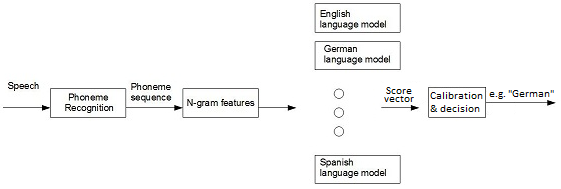
\includegraphics[width=\textwidth]{figures/prlm.png}
	\caption{Block diagram of a PRLM system, based on \cite[Fig. 41.5]{lidbok}}
	\label{fig:prlmoverview}
	\end{center}
\end{figure}

Another design for language recognition systems shown in figure \ref{fig:vscoverview} is based on an utterance's Vector Space Characterization (VSC). The technique is inspired from the information retrieval community where documents are represented by a document vector \cite[p. 826]{lidbok}. For language recognition systems we can construct spoken document vectors from the counts of $n$-grams in an utterance. If the distribution of $n$-grams is different for languages, then the documents for languages will lie in different regions of the document space. A classifier can then recognize languages based on the region that a document vector is situated in. The size of the document vectors will grow exponentially with $n$, often resulting in a sparse document vector of a very high dimension. This often makes it possible to reduce the dimension of the document vectors without the document space losing its discriminative power. An example of such dimensionality reduction is iVectors, which is the topic in section \ref{sect:ivecttheory}

\begin{figure}[hbt!]
	\begin{center}
	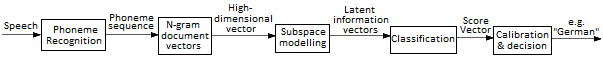
\includegraphics[width=\textwidth]{figures/vsc.png}
	\caption{Block diagram of a VSC language recognition system. The use of dimensionality reduciton is optional.}
	\label{fig:vscoverview}
	\end{center}
\end{figure}

It would be possible to construct the two systems using rules to recognize languages. The approach taken by many recent language recognition systems is to build a statistical model from training data. Without speculating on how much time it would take to create a rule based system, a statistical driven system should at least be easier to extend to new languages.


\section{Phoneme Recognizers}
\label{sect:phnrec}

In a PRLM or VSC recognition system, we first transform the speech signal to a phoneme sequence or string. This is done by a phoneme recognizer. With the many-to-one mapping by the phoneme recognizer we hope that there still is enough information about the language identity of the utterance, while the computational requirements for further processing will benefit from the reduced complexity of the problem. Even though each language uses its own set of phonemes, it is not necessary to train the phoneme recognizer to identify phonemes from all languages. This is because the phoneme recognizer doesn't need to make an correct transcription for an utterance, the system just needs the transcripts to be sufficiently distinct for each language \cite[p. 818]{lidbok}. For this reason it is possible to train the phoneme recognizer on a single language, which even may not have to be in the set of languages we are recognizing. Phone recognizers can utilize many of the techniques used in speech recognition,  where words often are recognized by their phoneme sequence \cite[p. 414]{talegk}. Here we will only present one such approach.

The speech signal is first split into short frames using a window function to reduce spectrum leakage \cite[p. 257]{talegk}. For each frame we can calculate the Mel-Frequency Cepstral Coefficients (MFCC). The transform takes the spectrum of the windowed signal through a set of filter banks that are spaced to approximate the Mel-frequency scale \cite[p. 314]{talegk}. After taking the logarithm of the filter outputs, we use the discrete cosine transform to get the cepstral coefficients. The whole process approximates the way the human auditory system responds to sound, which means that it should be suited for automatic phoneme recognition as well \cite[p. 314]{talegk}. Patterns in the cepstral coefficients when uttering a given phoneme can then be learned using labeled training data to train Gaussian Mixture Models (this is presented in section \ref{sect:backendscoring} for recognizing score-vectors).

The size of each frame is limited, in order to make the speech signal in each frame approximately stationary, but this doesn't mean that the neighboring frames have no information about the phoneme uttered in the current frame. Many recent phone recognizers use long temporal context techniques to capture the evolution of the signal outside of the frame \cite[p. 8]{butphnrec}. One such technique is to concatenate the $n$ cepstral coefficients in the current frame together with the $k$ past and future frames \cite[9]{butphnrec}, resulting in a $n(2k+1)$-dimensional feature vector. The high number of parameters in the long temporal context feature vector can make it difficult to train the phoneme recognizer without having huge amounts of training material. By assuming that the coefficients in past frames are independent of future frames, we can split the vector into a left and right context. This enables us to first classify each context separately, and then merge the results into a final decision of what phoneme was spoken \cite[p. 36]{butphnrec}. We can use Gaussian mixture models \ref{sect:backendscoring} for both classifying steps. The halving of the feature vector then increases the probability of observing similar features in the training set, reducing the need for much training data.

It is also possible for the phoneme recognizer to give multiple hypoteses for the phonemes used in an utterance. Such phoneme recognizers are said to be lattice based. Intuitively a lattice based phoneme recognizer will keep more of the information from the original speech signal, and has been shown to improve the performance of many language recognition systems \cite[p. 818]{lidbok}.


\section{Language Models and Classifiers}
\label{sect:basiclangmodel}

The responsibility of a language model or classifier is to output a single score per language from the phoneme sequence $S$. Since our final recognition decision will be based on the probability that an utterance belongs to a language, $p(l_i, | S)$, it seems natural to want the scores to approximate that probability. This is a somewhat strict requirement for systems as described in section \ref{sect:sysoverview} since the scores will be further processed by the backend. At the very least, a good language model should give scores that are easily transformable to an estimate of this probability. 

In order for the system to perform well for languages with limited available training data, it will be beneficial that the system is easily trained. A too complex classifier or language model will not be able to see patterns in the data, it will instead be over-fitted to explain each utterance independently which makes it unfit to score utterances outside of the training set \cite[p. 311]{information}. Over-fitting can be reduced by using a larger training set \cite[p. 147]{machinelearningbook}, but it is clearly an undesirable feature for language models. This is also the reason why we need a separate data set to evaluate the recognition system. The systems recognition performance on the data it was trained for will not necessarily extend to unseen data.

If we introduce the notion that training and test data are generated from a random process, the system's ability to correctly estimate $p(l_i | S)$, and thereby make correct recognition decisions, will be given by two error sources called model \emph{bias} and \emph{variance} \cite[149]{machinelearningbook}. \emph{Bias} is high if the system consistently over- or underestimate $p(l_i | S)$ for some documents regardless of the training set. In this way it represents the systems inability to correctly predict certain documents. Model \emph{variance} is the variance in the probability estimate of an utterance belonging to a language when the model is trained with different data. It represents the systems sensitivity to noise in the training data. Over-fitting is a symptom of a high variance system where the model is only expected to give correct probability estimates for utterances that are very close to a training utterance. A system with limited training data can generally not have both low variance and bias \cite[312]{information}, so a concession between the two errors has to be made.

%This was only a shallow introduction to language models due to the variety of techniques used in language recognition systems. A more detailed survey will be given when we discuss specific language models in section \ref{sect:basetrain} and ???.

\section{Backend Calibration of Score Vectors}
\label{sect:backendscoring}

The backend will calibrate the scores from the classifier or language model into the posterior, $p(l_i | S, \theta)$, so that so that they can be applied to the recognition decisions discussed in section \ref{sect:detvsid}. This calibration can also be trained using real data. A separate calibration step allows us to ignore application dependent information like what other languages should the system recognize, and the prior probability of a user speaking each language. The language models for each language can then be trained independently since it only needs to return some number that in some way correlates with the posterior probability for its language. Even if the language model is trained to return estimates of the posterior, there may still be some benefits calibrating the score vectors \cite[p. 820]{lidbok} as there might exist patterns in the scores that can be exploited. Furthermore, the back-end can be used to fuse scores for an utterance from multiple systems using different phoneme recognizers or language models. The fused system is then expected to perform better than each of the individual systems as long as the errors each system makes are somewhat uncorrelated \cite[p. 818]{lidbok}.

\subsection{Gaussian Backend}
\label{sect:gmmscore}

It is likely that the best calibration method will depend on the nature of the score-vectors given from the language models. A very flexible tool to perform calibrations that impose little demands on the score vector is to use a multivariate Gaussian mixture model (GMM). With this framework, the score vector, $\mathbf{y}$, for a given language is assumed to be produced from a generative statistical model. The likelihood of a $r$-dimensional Gaussian component $k$ to produce a score vector $\mathbf{y}$ is then

\begin{equation}
\label{gmmeq}
p(\mathbf{y} | \mathbf{\mu}_k, \mathbf{\Sigma}_k, K = k) = \frac{1}{(2\pi)^{r/2}|\mathbf{\Sigma}_k|^{1/2}}\exp(-\frac{1}{2}(\mathbf{y}-\mathbf{\mu_k})^T\mathbf{\Sigma}_k^{-1}(\mathbf{x}-\mathbf{\mu_k}))
\end{equation}
where $\mathbf{\mu_k}$ is the $r$-dimensional mean of the score vectors produced by the mixture, $\mathbf{\Sigma}_k$ is the covariance of the mixture and $|\mathbf{\Sigma}_k|$ its determinant \cite[p. 94]{talegk}. From Bayes rule we have that
\begin{align}
p(K=k | \mathbf{\mu}_k, \mathbf{\Sigma}_k, \mathbf{y}) &= 
\frac{p(\mathbf{y} | \mu_k, \Sigma_k, K= k) \cdot p(K=k )}{p(\mathbf{y})} \nonumber \\
&= \frac{p(\mathbf{y} | \mu_k, \sigma_k, K=k) \cdot p(K=k)}{\sum_{\forall i \in K} p(\mathbf{y} | \mu_i, \Sigma_i, K=i) \cdot p(K=i)} \label{gmmchoose}
\end{align}
where $p(K=k)$ is the prior probability of the score vector being generated from mixture $k$. If we know what mixture each score vector in a training set belongs to, then $\mathbf{\mu}_k$ can be estimated as
\begin{equation}
\label{muest}
\mathbf{\mu}_k = \operatorname{E}(\mathbf{y} | \mathbf{y} \in k)
\end{equation}
and $\mathbf{\Sigma}_k$ as
\begin{equation}
\label{sigmaest}
\mathbf{\Sigma}_k = \operatorname{E}\left( (\mathbf{y}-\mathbf{\mu}_k)(\mathbf{y}-\mu_k)^T | \mathbf{y} \in k \right)
\end{equation}
where $E(a|b)$ is the conditional expectation \cite[p. 94]{talegk}. The power of the Gaussian mixture model we have now described is that it is enable to model any probability distribution \cite[p. 95]{talegk}, which means that it is applicable to any type of score-vector. Even for a training set, we will generally only know the language of an utterance, but not the mixture the score vector belongs to. This means that equation \ref{muest} and \ref{sigmaest} cannot directly be solved. We can still estimate the parameters using the iterative EM-algorithm \cite[p. 439]{machinelearningbook}. With one mixture per language, equation \ref{muest} and \ref{sigmaest} can be solved by noting that $\mathbf{y} \in k$ is equivalent to that the score vector stems from the given language, $l_i$, and $p(K=k)$ is the prior for the language. We can then use $p(L=l_i | \mu_i, \Sigma_i, \mathbf{y})$ given in equation \ref{gmmchoose} to label unknown utterances.

